% Report Template
% Compile with XeLaTeX
\documentclass[a4paper,11pt]{article}
% \usepackage{fontspec}
% \setmainfont{EB Garamond}
%
\usepackage{amsmath}   %Better maths and more symbols
\usepackage{textcomp}
%
\usepackage[margin=1.5cm]{geometry}  %set margin width all around page
\usepackage{setspace}
\usepackage[compact]{titlesec}
%
\usepackage{graphics}
\usepackage{graphicx}
\graphicspath{ {img/} }  %Graphics saved in same directory as .tex file
\usepackage{float}  %Fancy graphics placement [H] [H!] arguments
%
\usepackage{caption}
%
\usepackage{multirow}  % Table cells spanning multiple rows
%
\usepackage{enumitem}    % Enumerated lists in the same format as bullet lists
%
\usepackage{natbib}    %Bibliography management  %Use author/date citations
\bibliographystyle{agsm}
\usepackage{url}
\usepackage{cite}
%
\usepackage{color}
\newcommand{\todo}[1]{\textcolor{red}{#1}}   % \todo{NOTE TO SELF WRITTEN IN RED}
%
\usepackage{lineno}
\linenumbers

%--------------------------------------------------------------
\begin{document}
%--------------------------------------------------------------
\setlength{\parskip}{10pt}   %space after paragraphs
\setlength{\headsep}{30pt} %space at page top
\setlength{\parindent}{0pt} %length of indent at start of par
%
\titlespacing{\section}{0pt}{*3}{*-0.1} %Position section titles  {indent}{*spaceabove}{*spacebelow}
\titlespacing{\subsection}{0pt}{*-0.5}{*0} %Position subsection titles  {indent}{*spaceabove}{*spacebelow}
\titlespacing{\subsubsection}{0pt}{*0}{*0} %Position subsubsection titles  {indent}{*spaceabove}{*spacebelow}
%
\pagenumbering{arabic}  %Add page numbering
%
\raggedright %align text to the left with long words taken to the next line
%--------------------------------------------------------------
\begin{center}{\LARGE{Changes in forest structure along an elevational gradient in the Peruvian Andes cause species-specific stress responses in tree seedlings}}\end{center}  %Insert Title

\section{Abstract}
4 bullet points (1) research conducted + rationale, (2) central methods, (3) key results, (4) main conclusions including key points of discussion. 

\section{Introduction}
Rapid anthropogenic climate change is causing many species, across a wide range of taxa, to shift their distributions in space \citep{Hughes2000, Parmesan2006, Chen2011}. \citet{Chen2011} estimates average latitudinal and poleward migration rates of \todo{NUM} and \todo{NUM}, respectively. For sessile taxa such as trees, range shifts occur as a result of differential recruitment and mortality over space, at the leading and trailing edges of their range \todo{REF}. Previous studies have suggested that the ability of tree species to respond to changes in mean annual temperature and precipitation regime will be important in determining species success over the coming century \citep{Colwell2008, Chen2011, Feeley2012}. Species responses may occur either in the form of adaptation, \textit{i.e.} changes in phenology, physiology and morphology, or through range shifts over space as species track environmental conditions (Bellard et al. 2012). Range shifts of plant species have been observed in many studies across the world \todo{REF}, while the number of studies documenting adaptational responses are few, potentially indicating that climate change is occurring so rapidly as to prevent effective adaptational responses. Predicting range shifts and more importantly the ability for species to shift their ranges across space has become an active field of research \todo{REFS FROM BELLARD 2012}. Understanding species range shifts can help conservation scientists to identify species and species assemblages at risk of extinction and can inform strategies to mitigate the effects of climate change on biodiversity and ecosystem functionality \citep{REF}.

The majority of efforts to predict future species range shifts as a conservation tool have used bioclimatic envelope models \citep{Pearson2003}. Bioclimatic envelopes are constructed by correlating current species range extent with the observed environmental conditions within those boundaries, then projecting spatially explicit climate trends into the future under different climate change scenarios to predict how species range boundaries will adjust in response (e.g. \citealt{Berry2002, Peterson2002, Thuiller2005, Araújo2006}) \citep{Sinclair2010}. When predicting range shifts and species success under a rapidly changing climate however, it is important to consider that range shifts driven by a single environmental variable like mean annual temperature may cause recruitment of individuals into habitats that are suboptimal in other senses, if range shifts outstrip acclimatory/adaptive potential \todo{REF}. In these suboptimal habitats, range shifts may lead to reductions in local and regional species richness (Colwell et al. 2008), changes in community composition \todo{REF}, ecosystem functioning (Bellard et al. 2012), and ecosystem service provision that are not predicted by bioclimatic envelope models (Dobson et al. 2011, Isbell et al. 2011). Bioclimatic envelope models have been criticised for making a number of gross simplifications \todo{REF}, \todo{INCLUDE EXAMPLES?}. Basic bioclimatic envelope models assume that the breadth of the realised niche (observed spatial range) equals that of the fundamental niche (bioclimatic envelope) (Jump \& Pe\~{n}uelas 2005, Hoffmann \& Sgr\`{o} 2011). This assumption is challenged by studies which demonstrate that the realised niche is often restricted, owing to the presence of unmeasured environmental pressures, such as biotic interactions with other species (Davis et al. 1998, Van der Putten et al. 2010, Ettinger et al. 2011). In order to accurately predict range shifts and their consequences for future biodiversity, it is important to expand bioclimatic envelope models to include variables which describe habitat as well as climatic variables such as temperature and precipitation, \todo{but this is as yet an understudied area of research.}

For forest trees, particularly in moist tropical forests, there are often high levels of mortality during the seedling recruitment stage, creating a demographic bottleneck \todo{Coomes and Grubb 2000}. Many seedlings perish due to suboptimal shade regimes created by the arrangement of adult trees \todo{REF}. The seedlings of many tropical tree species are highly adapted to shade \todo{REF}, meaning that if a seedling germinates in an open space, mortality by UV damage to photosynthetic machinery is quite probable. Seedlings may also compete with adult trees for nutrients \citep{}, although there is some separation between seedling and adult tree rooting depths for most species \citep{}, especially for the largest trees \citep{}. This mortality bottleneck provides a limiting factor to the success of tropical forest tree species experiencing range shifts. If seedlings germinate in areas that are only sparsely shaded, UV-B damage may occur leading to loss of photosynthetic capacity \citep{}, reducing growth rates and occasionally resulting in seedling mortality \todo{REF}.  

In montane cloud forests, range shifts are occurring more rapidly than in other areas \citep{} \todo{WHY?}. As mean annual temperatures rise, plant species are being figuratively pushed up-slope, with higher recruitment at the upslope edge of their range and higher mortality at the downslope edge of their range \citep{}. Particularly in the tropics, as altitude increases, UV-B concentration increases, with many species found at high altitudes \todo{REF} having specific adaptations to avoid UV-B damage to photosynthetic machinery, such as \todo{WHAT?}. Species found at low altitudes however, are less adapted to high UV-B environments, instead having adaptations to make the most of the diminished light levels found under thick tree canopy, particularly during the seedling growth stage \todo{REF}. It therefore follows that as lowland species move upslope in response to increasing temperature, they may experience increased levels of damaging UV-B radiation as the canopy thins, but little research has been devoted to this aspect of elevational range shifts.  

\todo{Do I need more here before I jump into ``this study''?}

In this study, we investigated the effects of variation in adult tree canopy structure and size distribution on seedling growth form and photosynthetic stress, across an elevational gradient in the Peruvian Andes, spanning lowland west forest and montane cloud forest. We tested three hypotheses: 1) Within a species, seedlings growing at higher elevations would experience higher levels of photosynthetic stress than those at lower elevations, 2) Species would differ in their degree of acclimation to variation in adult tree canopy structure and size distribution, 3) A combination of biotic and abiotic explanatory variables would best explain variation in seedling morphological and physiological traits across their elevational range.  

\section{Materials and Methods}
\subsection{Study Site}
Data collection was conducted across 10 permanent 1 ha forest plots in the Kos\~{n}ipata Valley of Man\'{u} National Park, Peru (-13\textdegree N, -71\textdegree W, Figure \ref{fig:sites}, Table \ref{table:sitechar}). The Kos\~{n}ipata Valley has been identified as a migration corridor for lowland species to migrate to higher elevations in response to temperature increase \citep{Feeley2011} and so is an appropriate location to study range shift drivers. Plots are situated between 400 and 3200 m.a.s.l. along this migration corridor (Table \ref{table:sitechar}, Figure \ref{fig:range_plot}). The plots form part of a larger plot network established by the Andes Biodiversity and Ecosystem Research Group (ABERG) in 2003 \citep{Malhi2010, Girardin2013a}, and are located within the "Tropical Andes" biodiversity hotspot identified in \citet{Myers2000}. The plots used in this study contain 719 tree species, and the valley as a whole contains 1167 tree species \citep{}.

\subsection{Study species} 
We chose nine tree species for comparison from a range of 1635 identified species within the 10 study plots. Species were selected according to their contrasting ranges (Figure \ref{fig:range_plot}), differences in genus migratory pattern \citep{Feeley2011}, and because each species is dominant across it's range in the Kos\~{n}ipata Valley \todo{(ABERG, unpublished data, Appendix VI)}. Despite having no quantitative range shift prediction information, Iriartea deltoidea and Dictyocaryum lamarckianum were included in order to observe potential differences in response between monocot and dicot species, as both are monocots. Both \textit{I. deltoidea} and \textit{D. lamarckianum} are large-seeded palm species, as such, they are expected to be migrating upslope, similar to other large-seeded palms \citep{Hillyer2010}. Seedlings of \textit{Myrcia spp.} are difficult to reliably identify to species in the field due to similar morphology and were thus sampled as a composite of three potential species: \textit{Myrcia splendens}, \textit{M. fallax}, and \textit{M. rostrata}, the only \textit{Myrcia} species known to be present in our plots from ABERG censuses. They are referred to as \textit{Myrcia spp.} from here on. 

\begin{figure}[H]
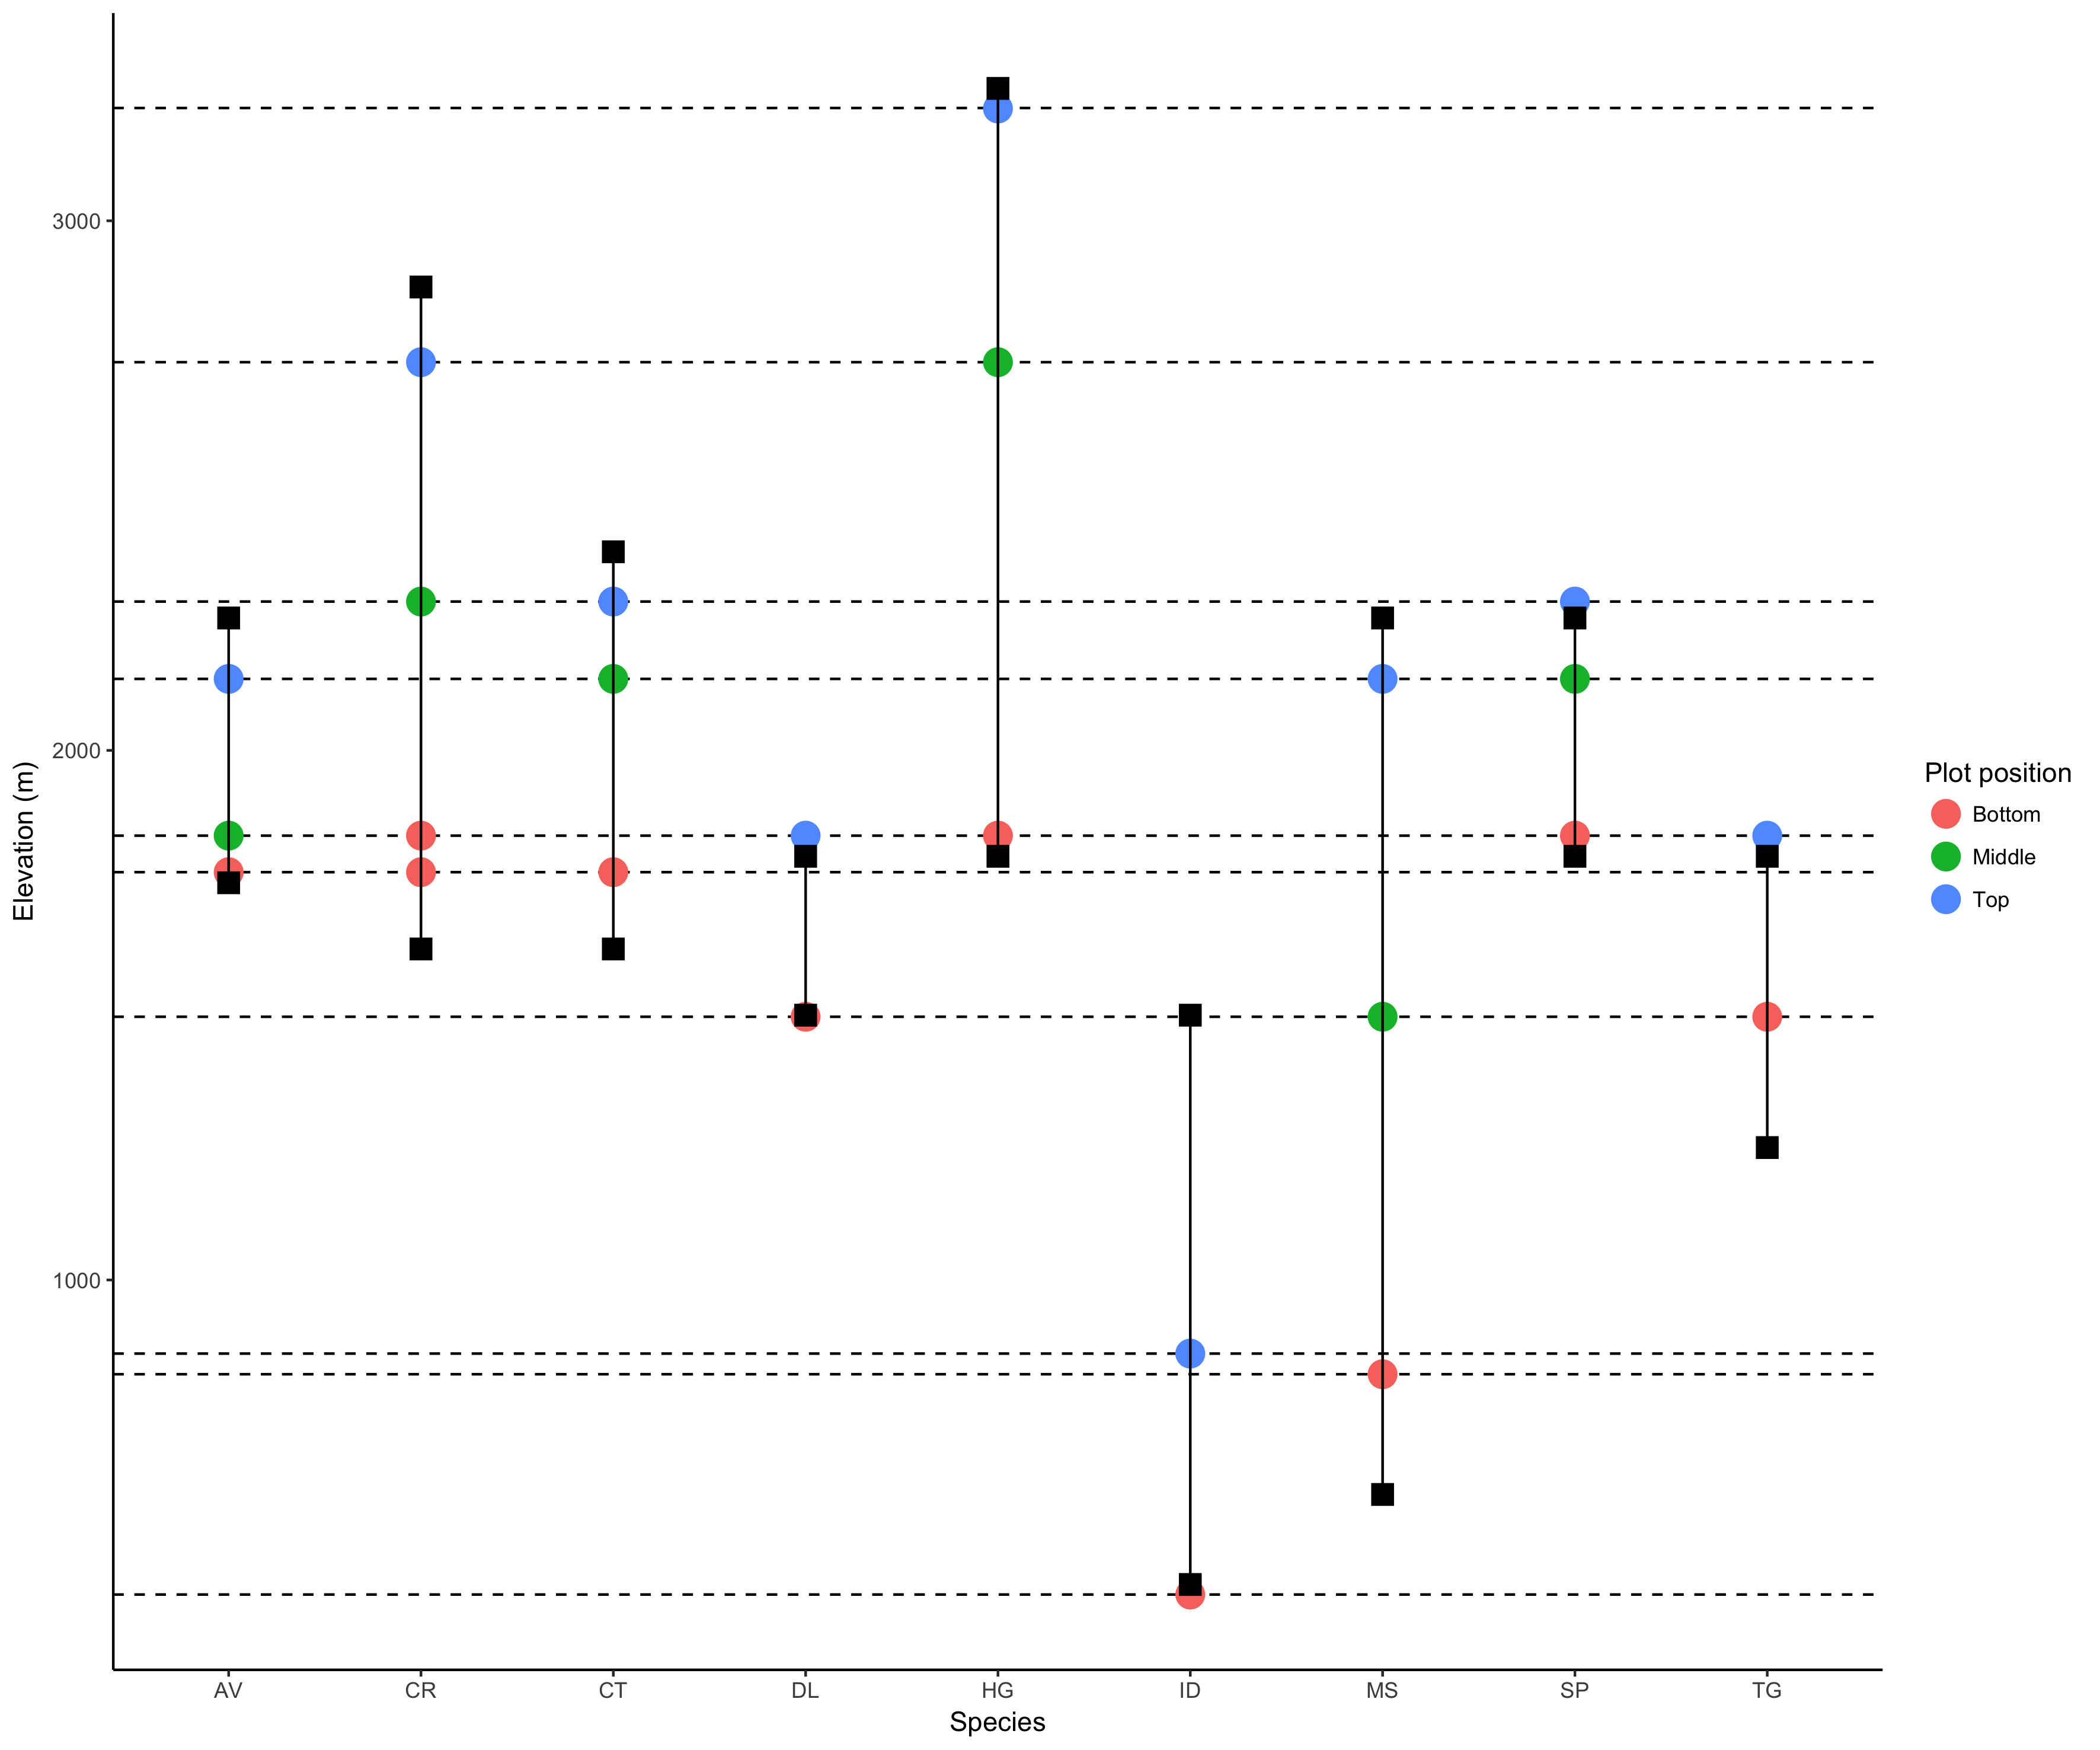
\includegraphics[width=\textwidth]{ranges_ggplot}
\centering
\caption{Elevation of study plots for each species (coloured points) with the upper and lower range extents for each species (black squares). Plot elevations are marked as dashed lines.}
\label{fig:ranges_ggplot}
\end{figure}

\subsection{Sampling and Measurement}
Species were sampled in three plots representing the upper, middle and lower elevational extents of their ranges (Figure \ref{fig:ranges_ggplot}). Within each plot, a maximum of 10 seedlings were sampled. Seedling mortality creates a narrow bottleneck for tree survival in closed canopy tropical forests, seedlings are particularly sensitive to environment stress. Previous studies have demonstrated seedling vulnerable to climate change \citep{REF}. \todo{something about dispersal not catching up at the same rate}. To minimise the chance of pseudo-replication of sampled seedlings, seedlings closer than 5 m to another seedling were excluded from the analysis, as it cannot be guaranteed that the stems are not connected by a stolon or rhizome, it also ensures that competition radius measurements are truly independent. Within a cluster of seedlings within 5 m of each other, each seedling was assigned a number and a random number table was used to choose a single seedling for measurement.

Proxies for photosynthetic efficiency \todo{or is it capacity???} were measured on the highest fully-expanded leaf of each seedling. Leaf photosynthetic efficiency can be used as an indicator of physiological stress levels. Plants with a lower photosynthetic efficiency are more stressed than those with a higher efficiency. Chlorophyll-\textit{a} fluorescence was measured using a Walz Mini-PAM II (Walz Effeltrich, Germany), on a randomly selected area of adaxial leaf surface, avoiding prominent leaf veins according to \citep{}. Chlorophyll-\textit{a} measurements were used to calculate F\textsubscript{v}/F\textsubscript{m} according to \citet{Genty1989}:

\begin{equation} \label{eq:fvfm}
F_v/F_m = (F_m - F_o)/F_m
\end{equation}

Where $F_m$ is the maximal fluorescence in the dark and $F_o$ is the minimal fluorescence in the dark \citep{Maxwell2000}. Fluorescence measurements were taken after exposing the seedling to 30 minutes of \todo{total} darkness, \todo{to ensure complete dark adaptation} \citep{Campbell2007}. Dark-adapted F\textsubscript{v}/F\textsubscript{m} measures the photosynthetic efficiency of the leaf by relaxing the reaction centres prior to the fluorescence measurement. F\textsubscript{v}/F\textsubscript{m} is preferable to other chlorophyll fluorescence measures as it removes the noise created by environmental conditions at the time of measurement, instead providing a measure of the underlying photosynthetic efficiency. A reduction in F\textsubscript{v}/F\textsubscript{m} is indicative of plant stress. Here, individuals with F\textsubscript{v}/F\textsubscript{m} values <0.7 are considered to be experiencing stress \citep{Maxwell2000}. 

In addition to F\textsubscript{v}/F\textsubscript{m}, leaf relative chlorophyll content was measured using a multi-spectral SPAD-meter (Minolta SPAD-502Plus, Spectrum Technologies, Plainfield, Illinois, USA). To account for variation in chlorophyll content across the leaf \todo{REF}, SPAD measurements were taken at three random points on the leaf. The mean of the SPAD values was used to calculate an estimate leaf chlorophyll content using the conversion factor outlined in \citep{}:

\begin{equation} \label{eq:chl-spad}
Chl = 0.53e^{\begin{matrix} 0.0364 \times SPAD \end{matrix}}
\end{equation}


\subsection{Leaf and whole-plant morphological measurements}

To assess adult-seedling competition interactions an adapted version of the Iterative Hegyi Index was implemented \citep{Hegyi1974, Lee2004, Seifert2014}. Our adapted `Iterative Seedling Index' (ISI) uses adult tree trunk diameter at \textasciitilde 1.3 m from ground level (Diameter at Breast Height, DBH) and the distance of trees from the seedling to calculate an index for each seedling, higher values indicate greater competition pressure from surrounding adult trees:

\begin{equation}
\label{eq:ISI}
ISI_i = log(\sum_{j=1}^n (\frac{1}{{DIST_i}_j} D_j))
\end{equation}

where $D_j$ is the DBH of a competitor tree and ${{DIST_i}_j}$ is the euclidean distance between seedling $i$ and competitor tree $j$. ISI was log transformed for analysis, as results spanned multiple orders of magnitude. The `iterative' aspect refers to the selection of competitor trees. An iterative selection method for competitive trees assumes that if the path between two trees is blocked, the intensity of competition between them will be greatly reduced \citep{Gadow1999}. The radius around the seedling is divided into 12 30\textdegree{} sectors, only the nearest tree \textgreater{}10 cm DBH within each sector is measured (Figure \ref{fig:hegyi}). The size of the competition radius ($C_R$) is defined as:

\begin{equation}
\label{eq:CR}
C_R = 2 \times \sqrt{\frac{10,000}{N}}
\end{equation}

where $N$ is the number of trees \textgreater10 cm DBH per ha (stand density). Stand density data was taken from ABERG census data within each plot (ABERG unpublished data) and used to interpolate values $C_R$ for plot VC, for which no stand density data exists, by fitting the elevation of the plot to a a linear regression between elevation and trees ha\textsuperscript{-1} for the remaining plots (\todo{Supplementary material}). $C_R$ was rounded to the nearest metre for ease of measurement (Table \ref{table:CR}). 

\subsection{Statistical Analysis}
A matrix of single predictor linear mixed effects models were compared to test for the presence and strength of the causal relationship between each competition variable and each plant trait. All model variables were standardised to allow easy comparison of effect sizes, according to \citep{Gelman2008, Grueber2011, Gelman2014}. Model quality was compared using Akaike Information Criteria ($AIC$) \citep{Akaike1998}, Akaike weights ($W_i$), and fixed effect pseudo-R\textsuperscript{2} values ($R_M^2$). 

The best quality single fixed effect models (using either independent intercepts or slopes for each species) were compared using $\Delta$AIC\textsubscript{r} against a random effects model,  the variance explained by the whole model ($R_C^2$) and the fixed effects ($R_M^2$), and slope coefficients (Figure \ref{fig:daic_r2c_traits}, Figure \ref{fig:slope_traits}) to compare their relative effect on plant traits. 

\todo{Add linear mixed model set up as an equation or schematic diagram or something}

To better understand the potential multiplicative effects of competition variables we also compared linear mixed effects models with combinations of fixed effects, using $AIC$, $W_i$ and $R_M^2$, to find the model which best explained variation in each plant trait.

To understand variation between species in their physiological and morphological response to competition effects, slopes for each species were calculated and compared in the linear models. 

In order to inform the error structure of mixed effects models, error structures of were compared using AIC values on pairs of single fixed effect linear mixed effects models, with a single plant trait response variable, where the slopes of each species were allowed to vary by either intercept or slope and intercept were compared to show whether species differ appreciably in their trait response to the various competition variables and elevation (fixed effects) (Figure \ref{fig:traits_dAIC}, Appendix III). Where $\Delta$AIC\textsubscript{rsri} scores between pairs of models are -2<$\Delta$AIC\textsubscript{rsri}<2 a random intercept structure is maintained, in order to maximise parsimoniousness. Models reported in the results use the optimal error structure according to AIC.



All statistical analyses were conducted using R, version 3.2.4 \citep{R2016}.

\section{Results}

\subsection{Variation in plant traits across elevation}

Physiological leaf trait models were not of a better quality when species were given their own slopes. All morphological traits had at least one model where a random slope structure for species produced a model of better quality. Leaf area was better using a random slope for all except herbaceous plant abundance.

Within each species, the degree to which plant traits varied over their elevational range differed significantly according to linear models of the effect of species on plant trait slope \todo{WHAT IS THE LINEAR MODEL RESULT? VARIANCE EXPLAINED} (Figure \ref{fig:interac_trait_elev_ggplot}, Figure \ref{fig:trait_elev_lm_scatter_ggplot}).

Single fixed effect mixed effects models were better than random effects models in 15/24 cases ($\Delta$AIC\textsubscript{r}>2) (Figure \ref{fig:daicplot_ggplot}).  However, competition variables account for only a small percentage of the variance in each plant trait, with the highest $R_M^2$ being ISI predicting stem volume ($R_M^2$ = 4.3\%) (Figure \ref{fig:r2plot_ggplot}). Elevation has a greater influence over plant traits than any competition variable in all cases.

\begin{figure}[H]
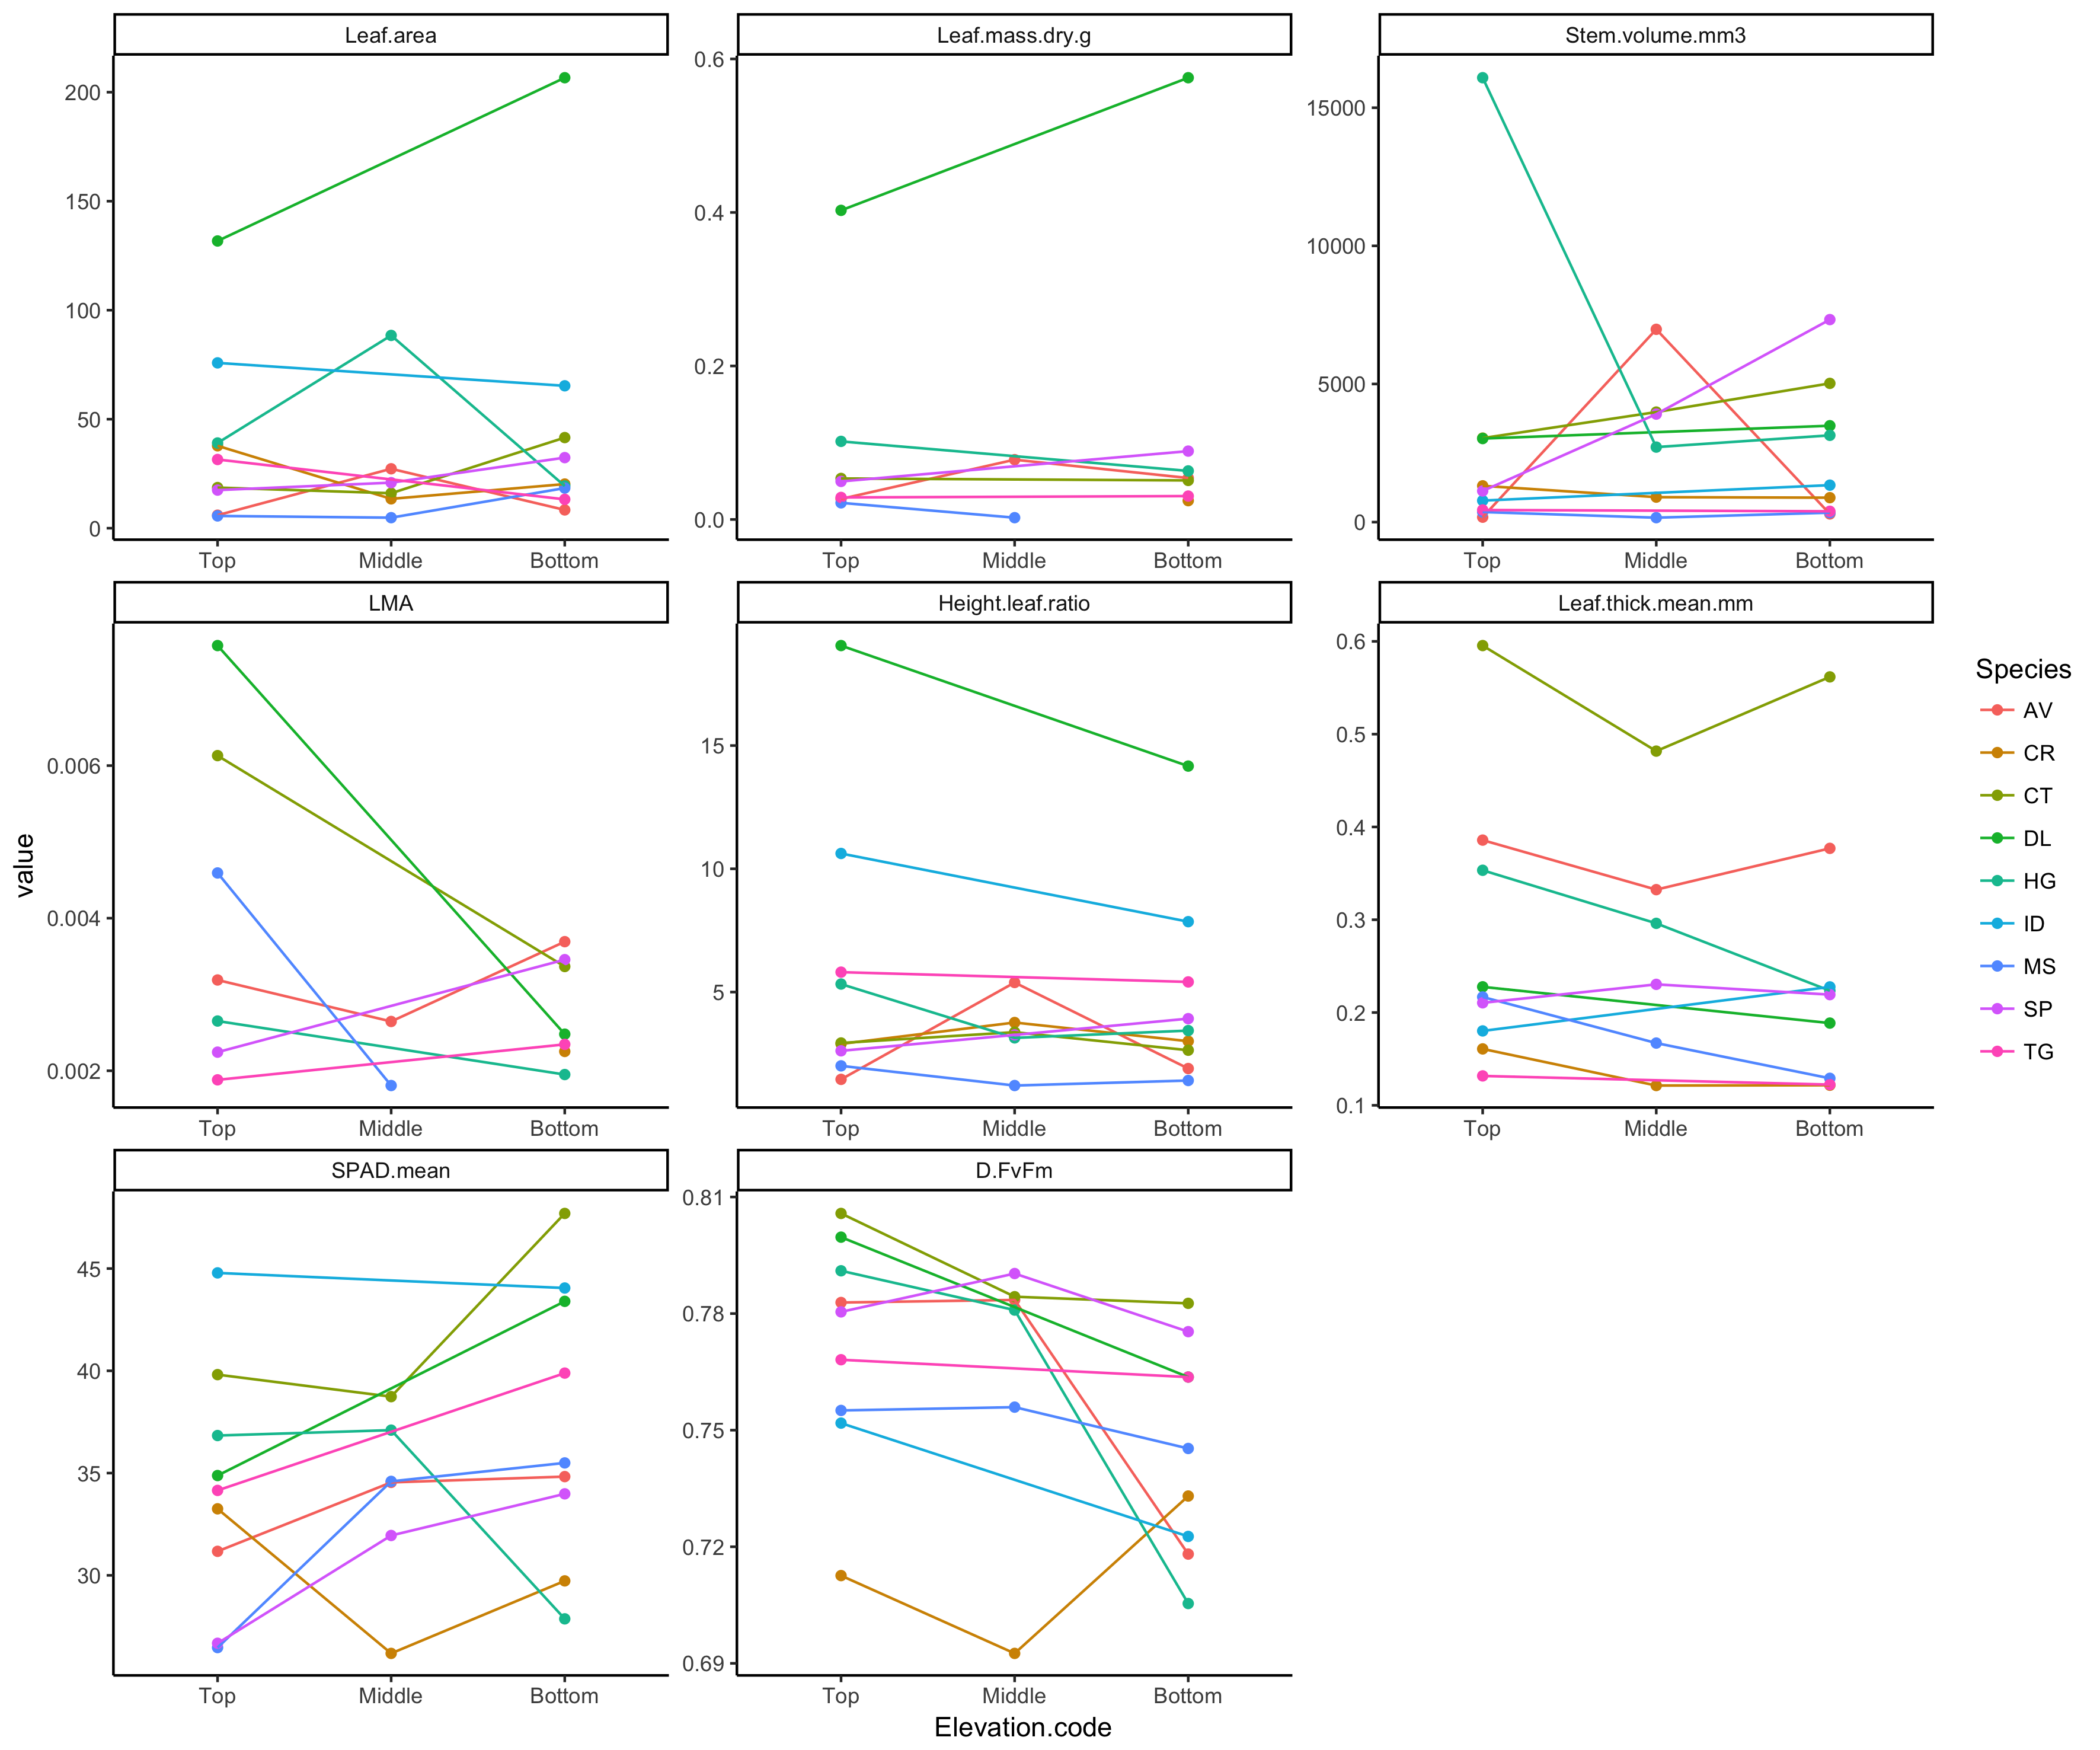
\includegraphics[width=\textwidth]{interac_trait_elev_ggplot}
\centering
\caption{Interaction plots showing the variation in plant trait values within each species.}
\label{fig:interac_trait_elev_ggplot}
\end{figure}


\begin{figure}[H]
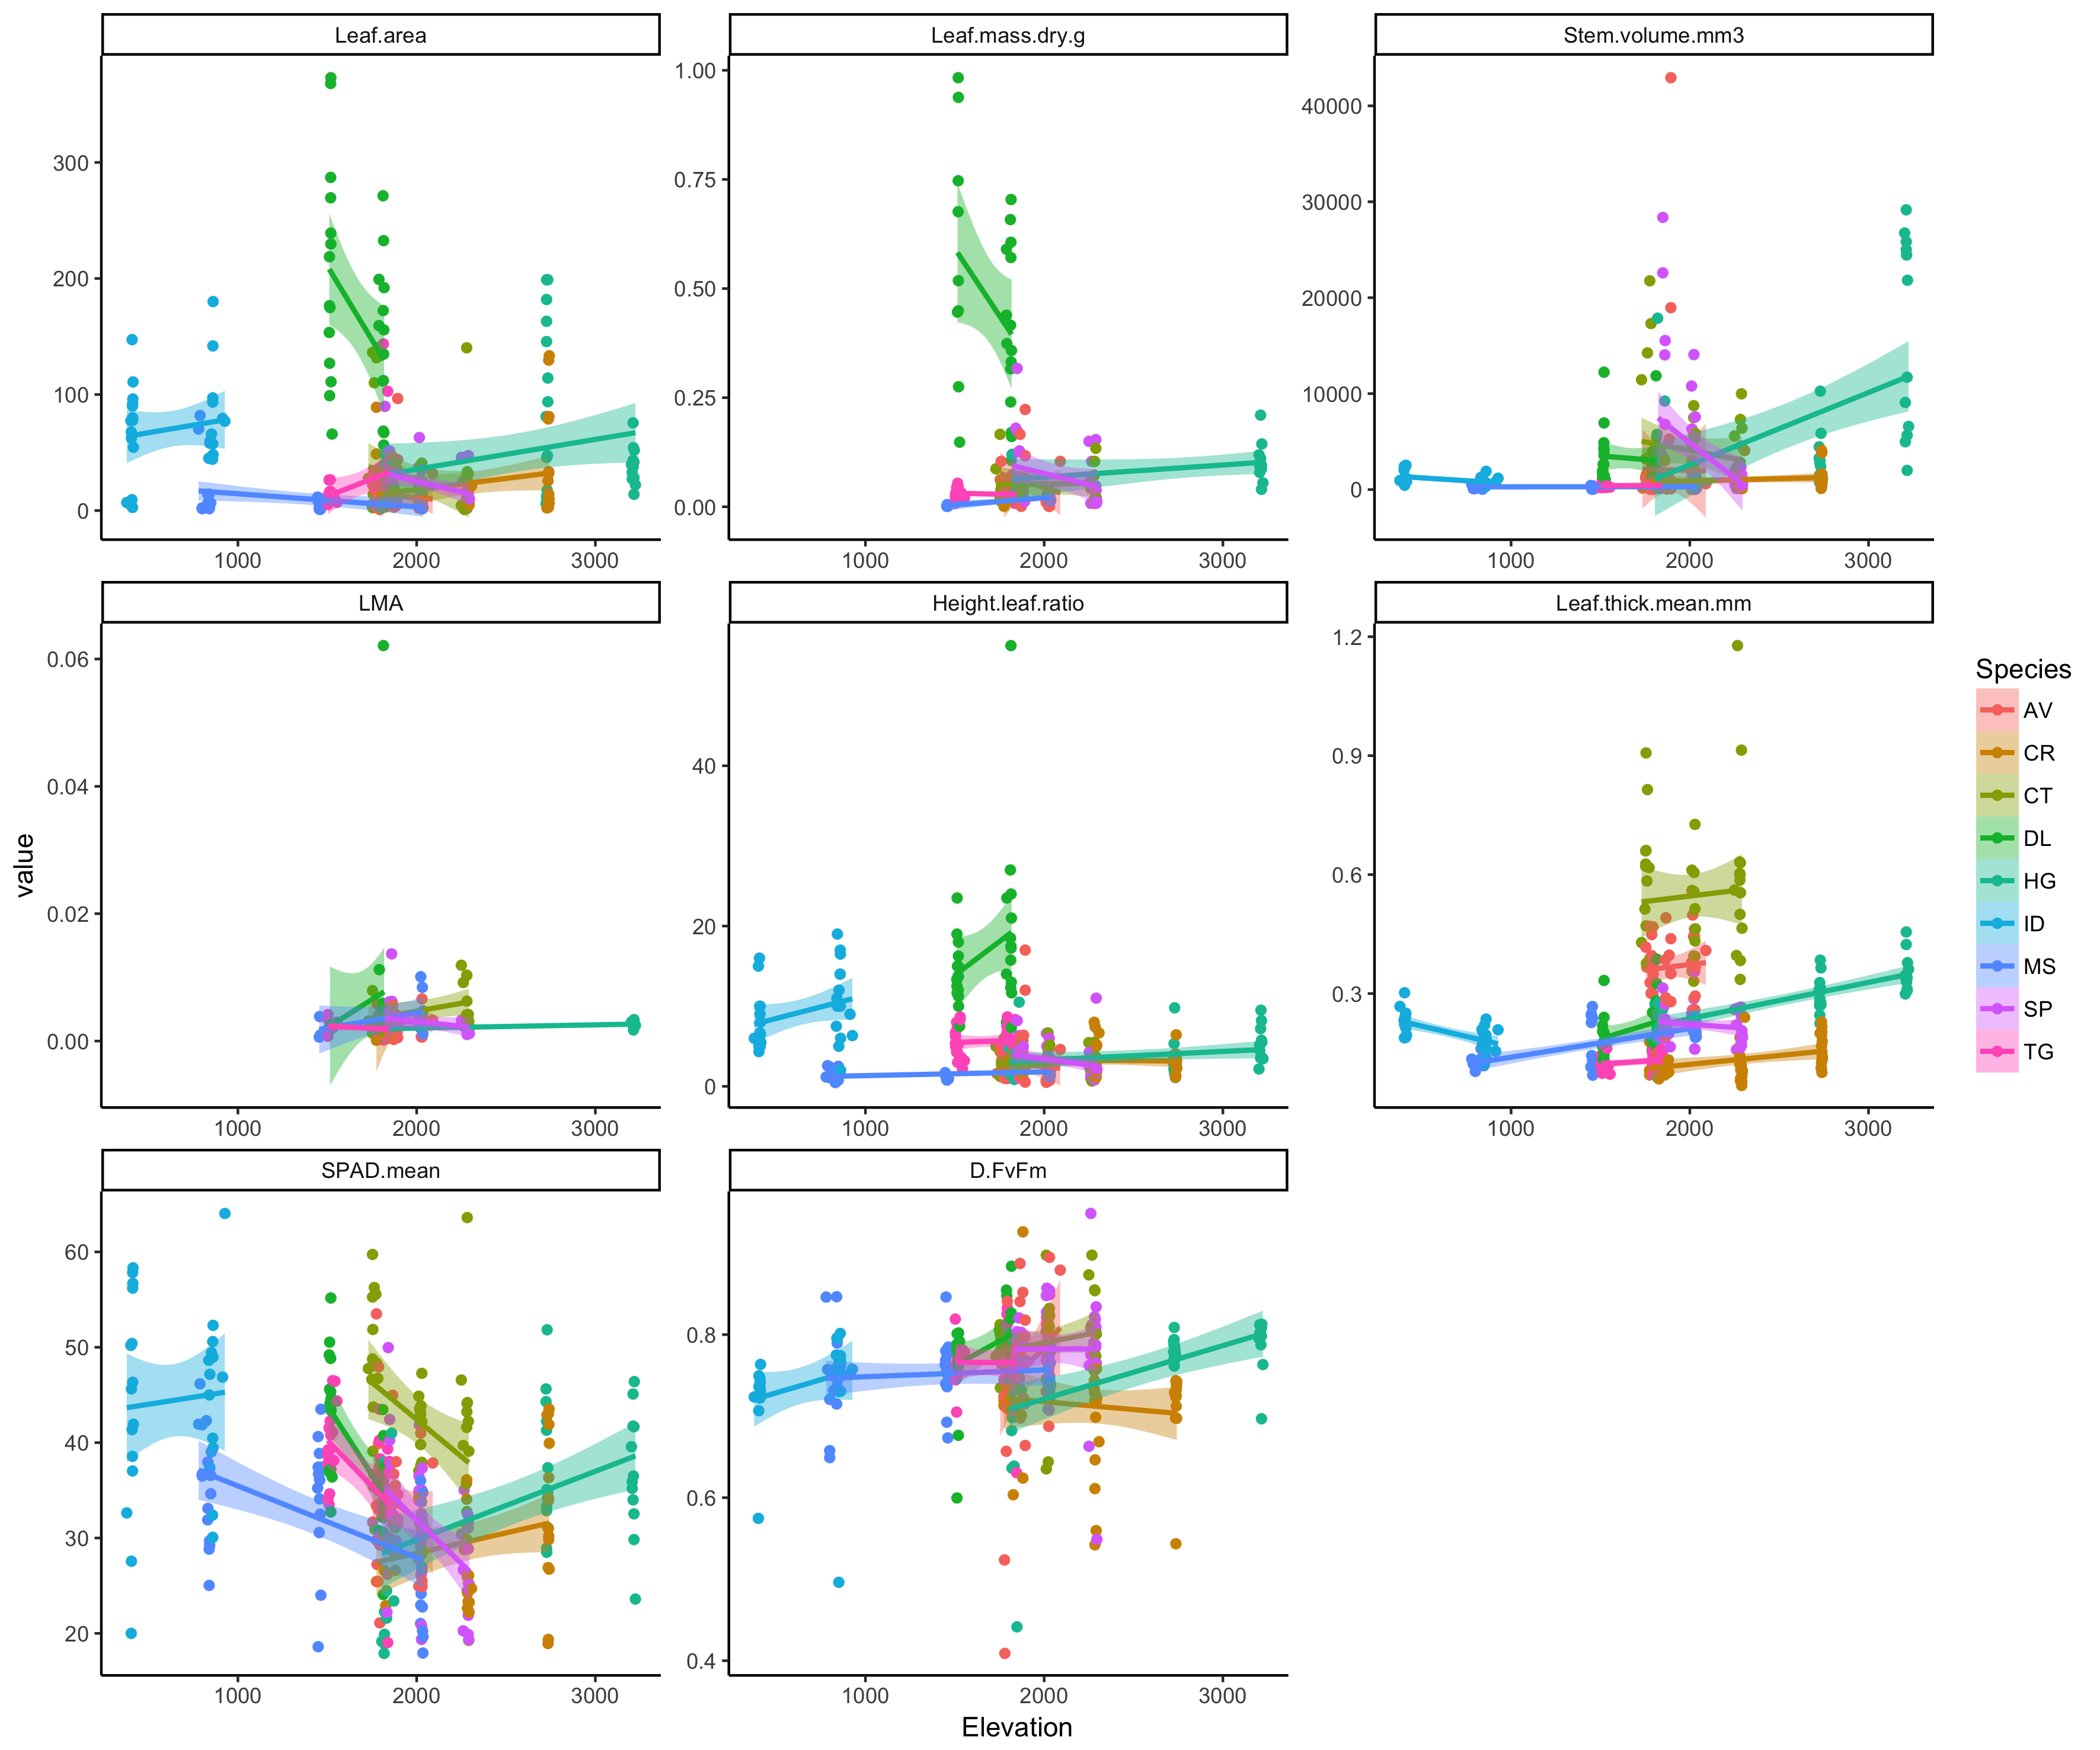
\includegraphics[width=\textwidth]{trait_elev_lm_scatter_ggplot}
\centering
\caption{Scatter plots with linear model fits for each species, showing the variation in plant stress variables and plant traits across elevation.}
\label{fig:trait_elev_lm_scatter_ggplot}
\end{figure}


\begin{figure}[H]
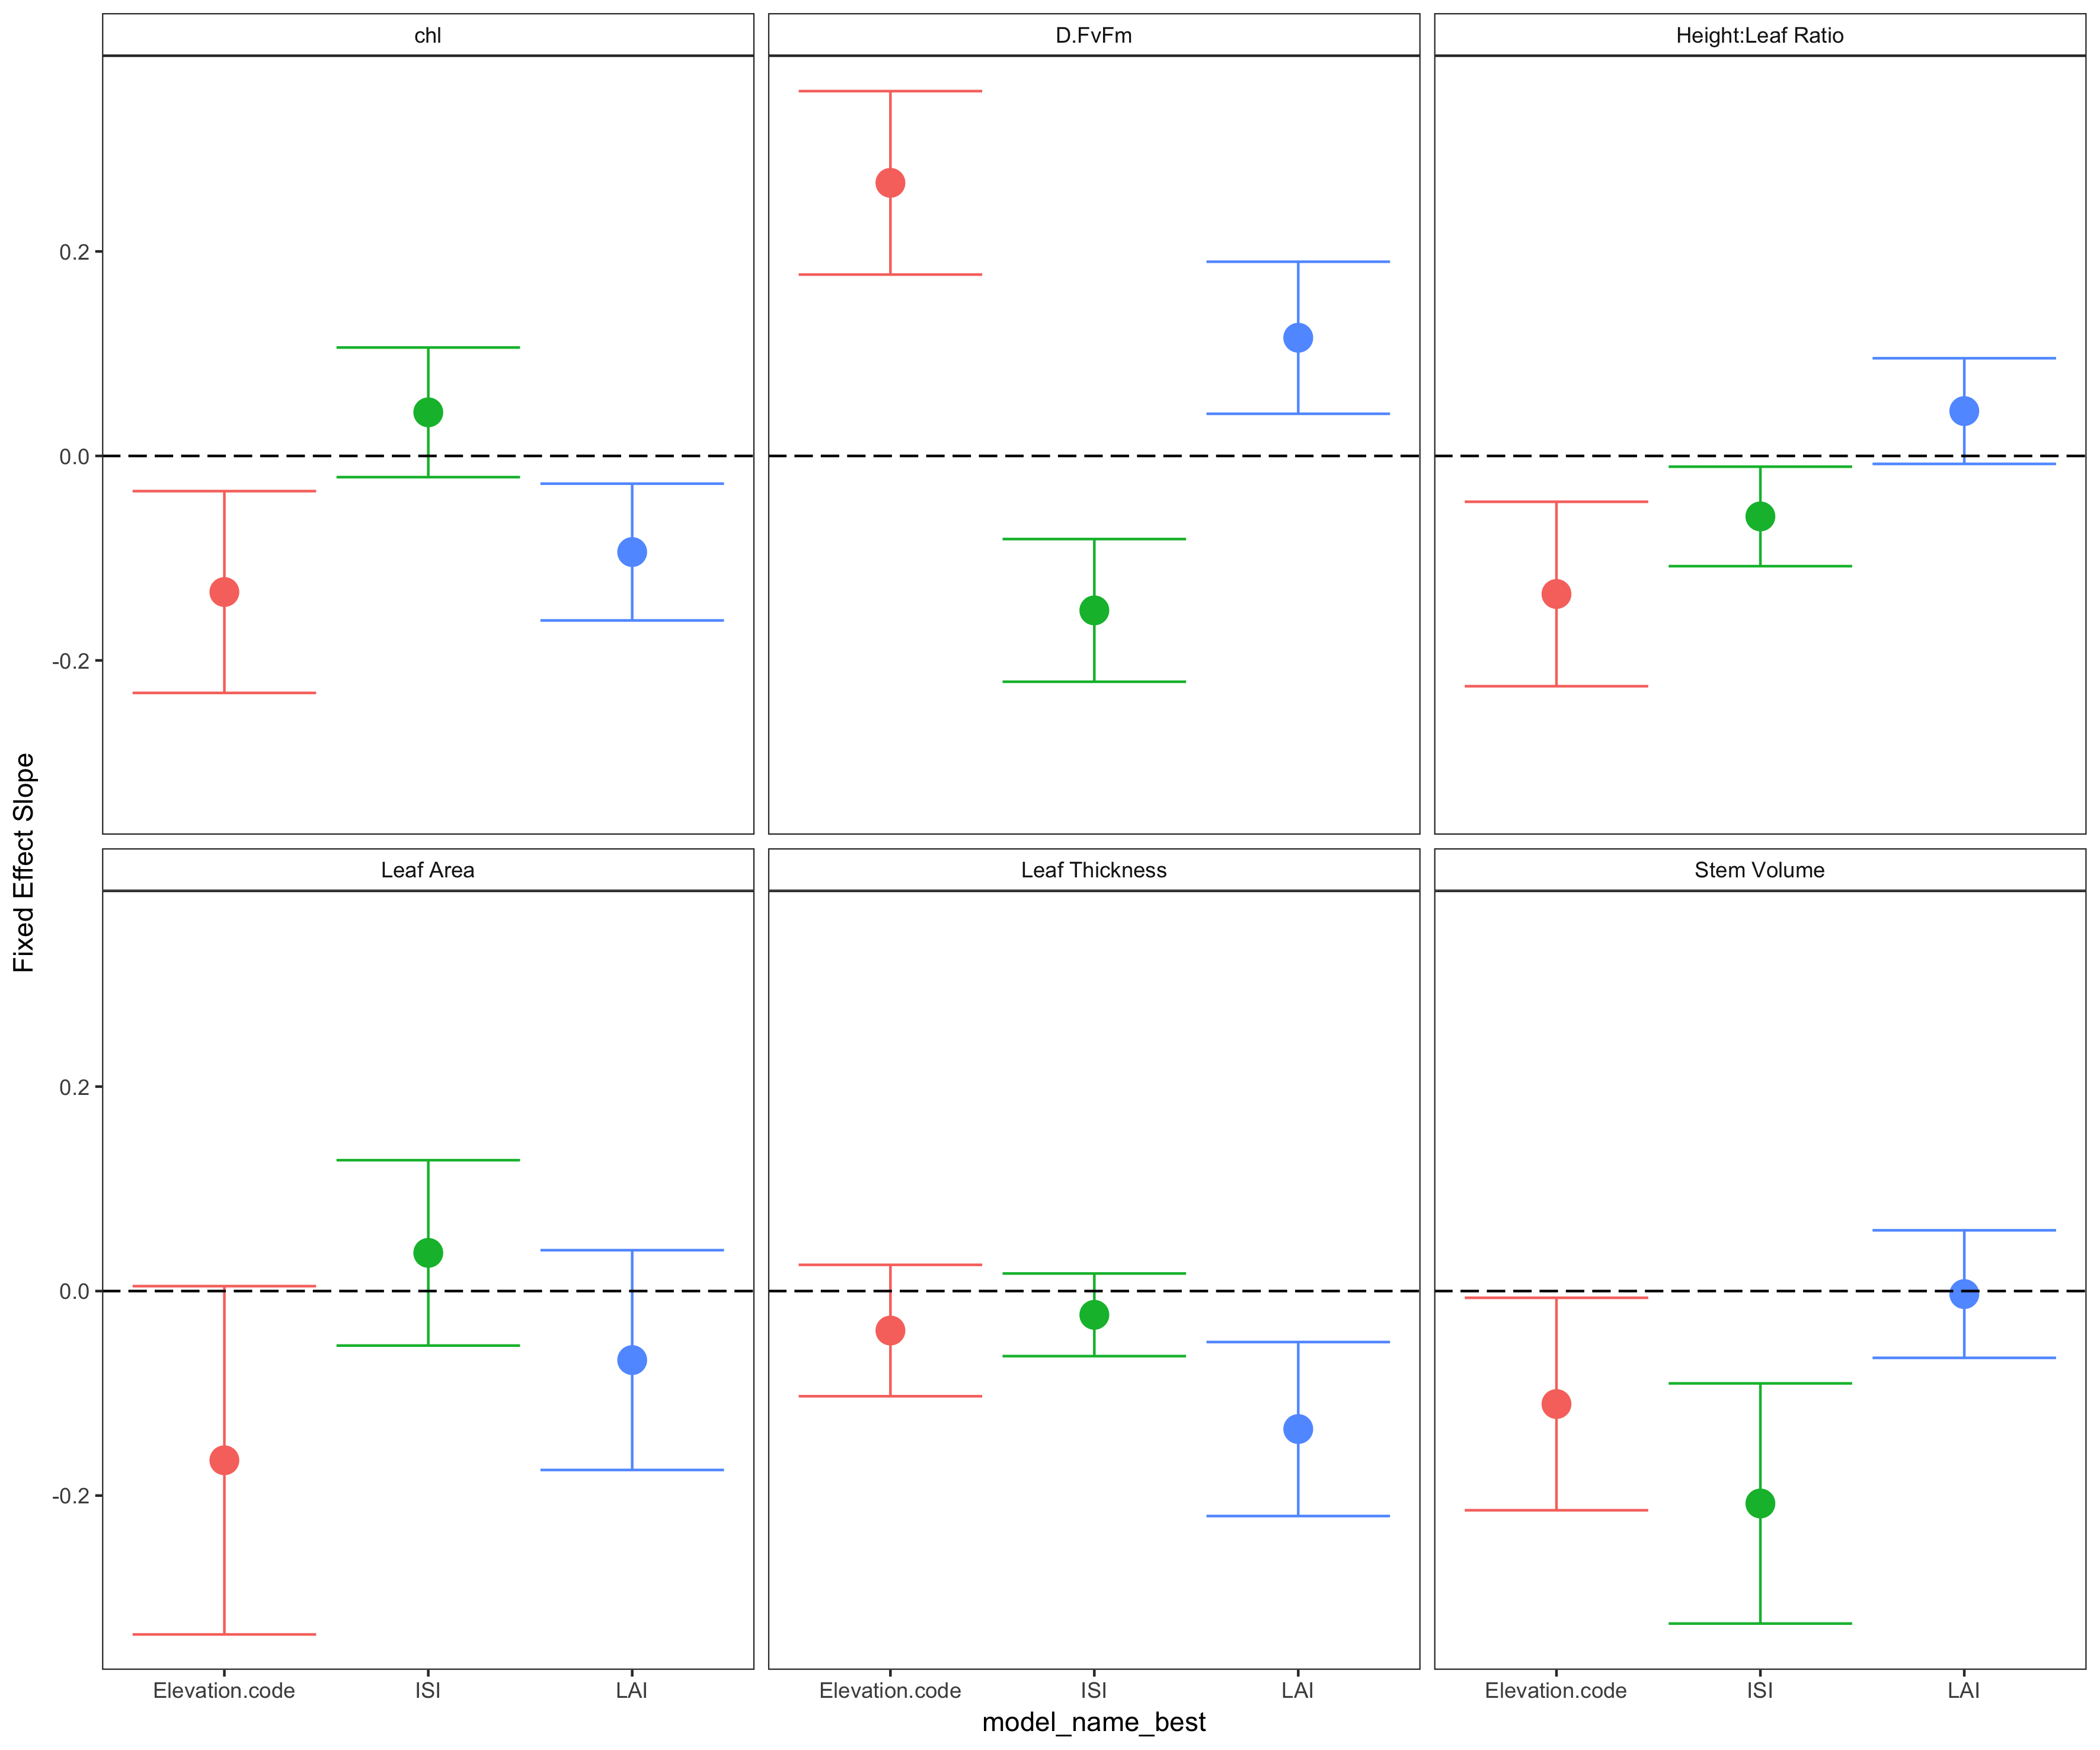
\includegraphics[width=\textwidth]{single_trait_eff_size_lmer_ggplot}
\centering
\caption{Interval plots showing the effect sizes (slopes) of each fixed effect in single fixed effect linear mixed effects models of plant traits against forest structure variables and elevation, for comparison.}
\label{fig:single_trait_eff_size_lmer_ggplot}
\end{figure}

\begin{figure}[H]
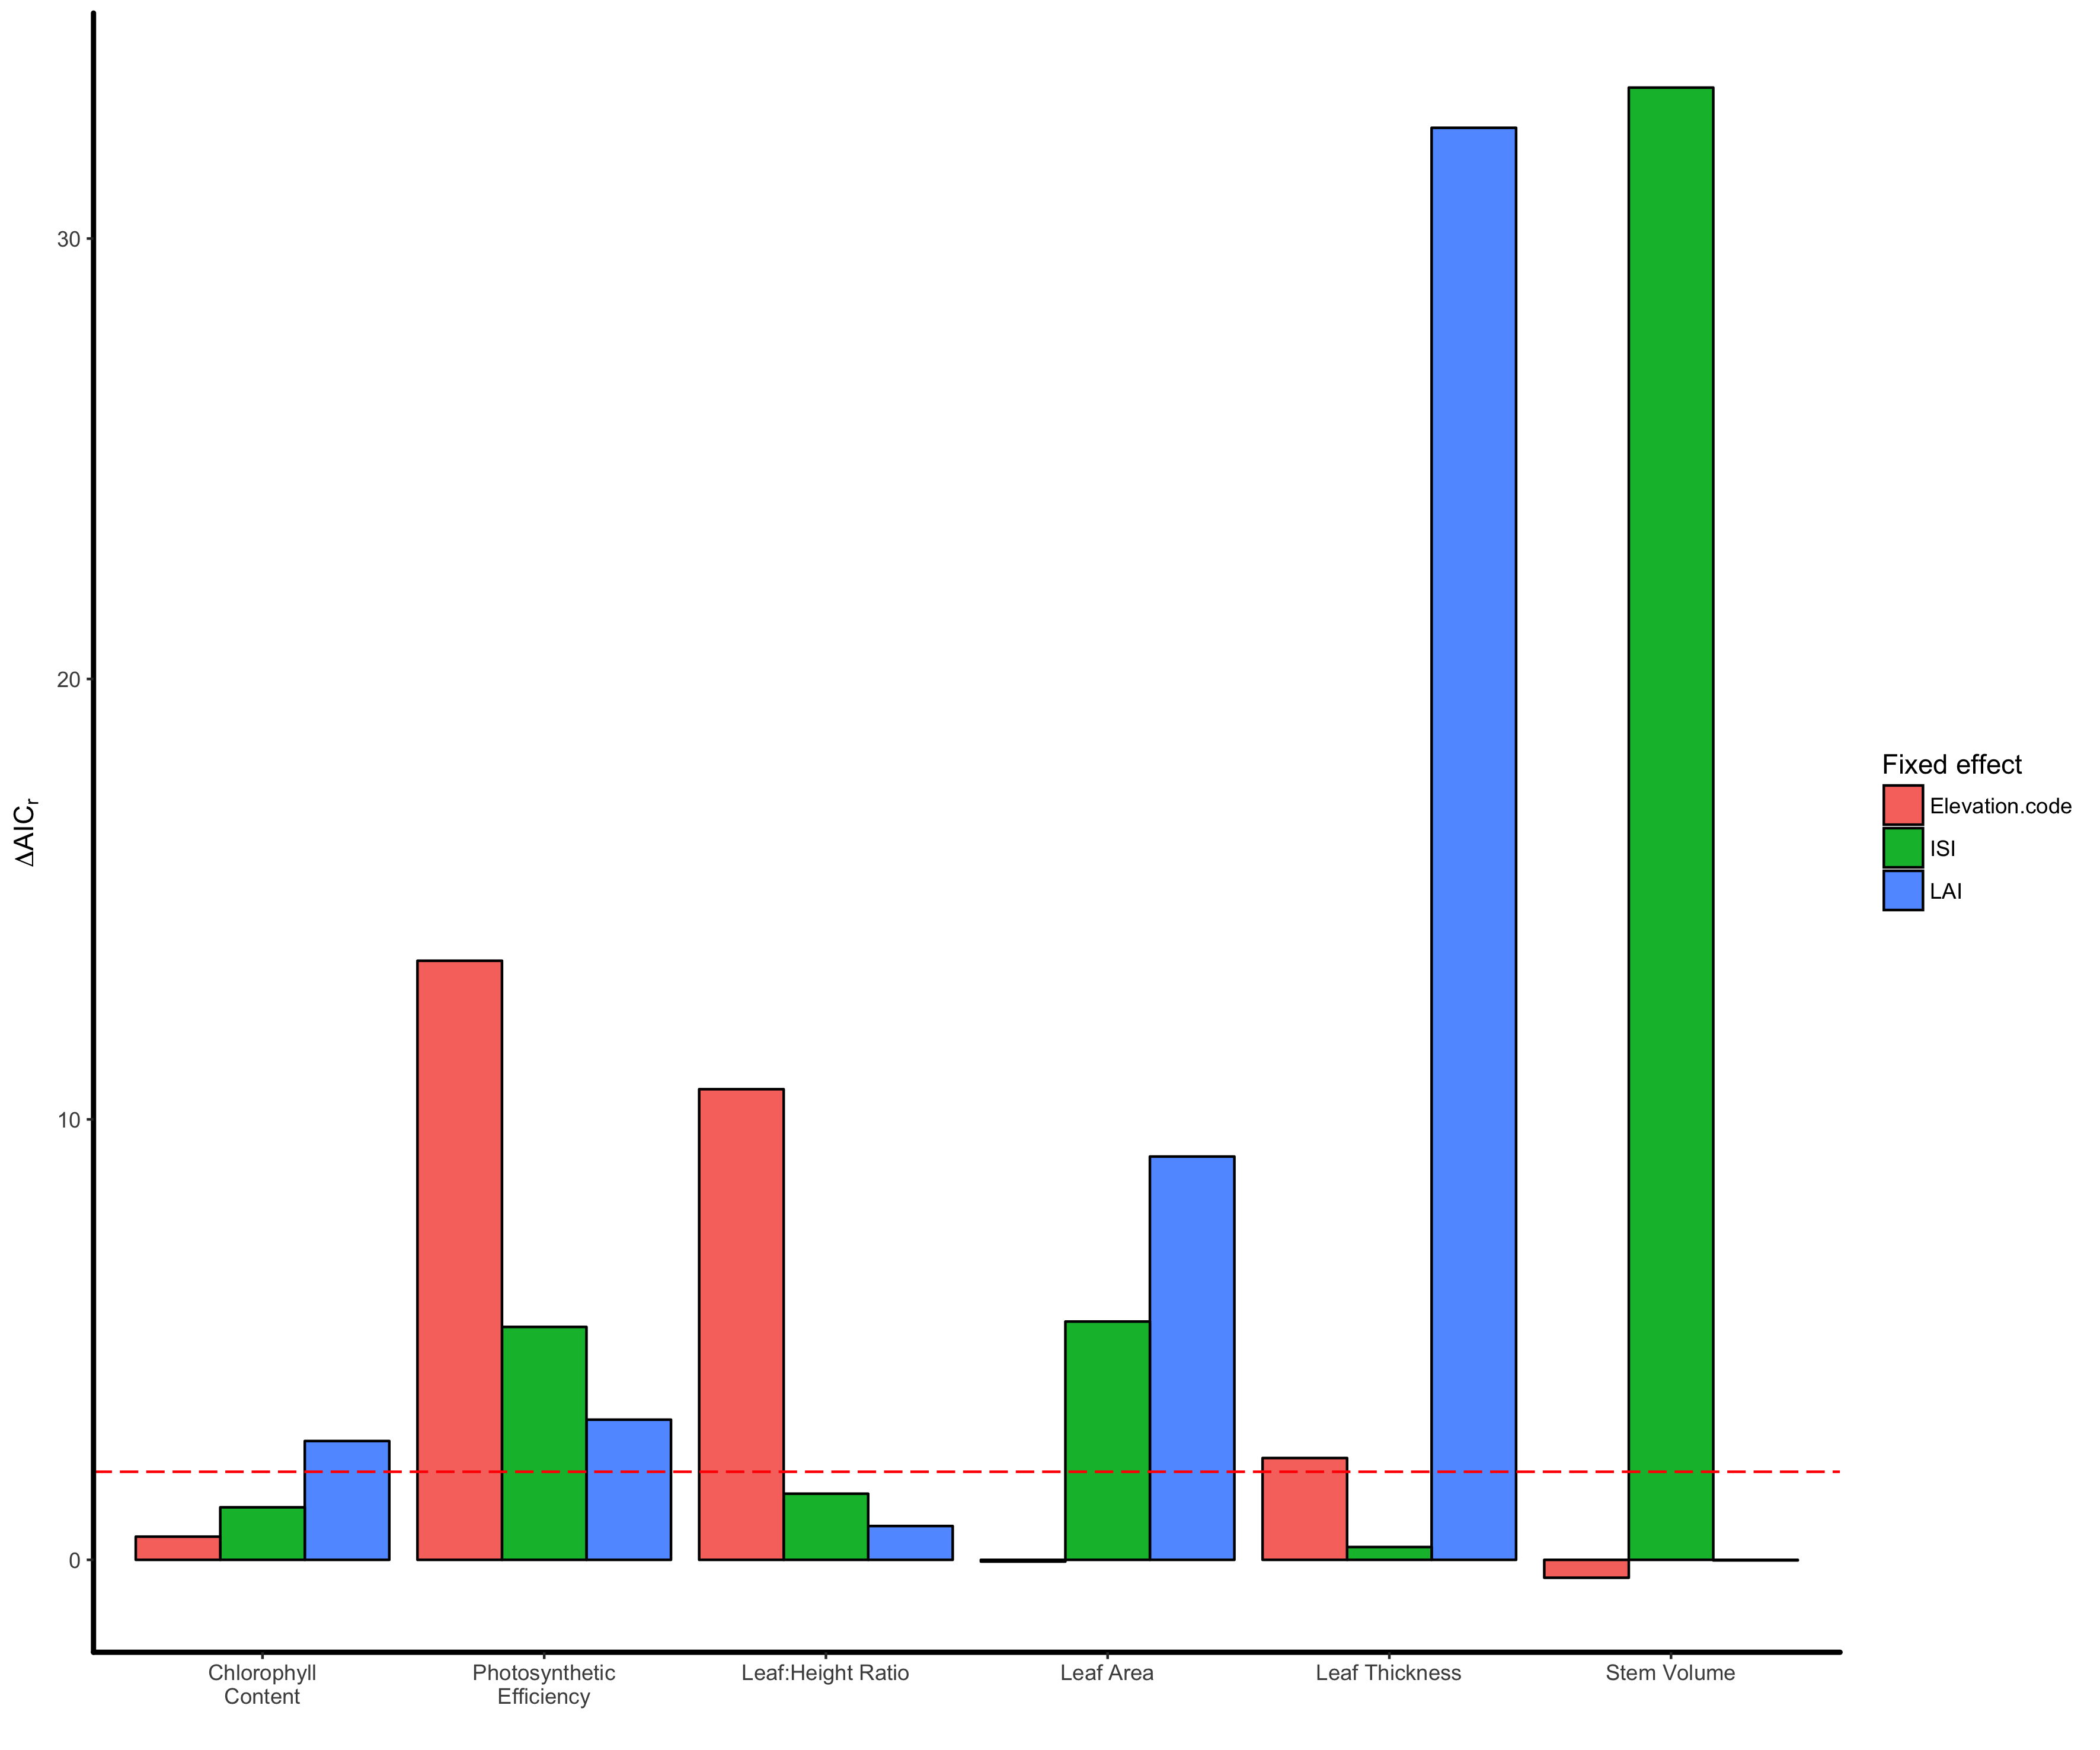
\includegraphics[width=\textwidth]{daicplot_ggplot}
\centering
\caption{The difference in AIC values between each single fixed effect model and a corresponding random effects model using no fixed effects. A higher $\Delta$AIC\textsubscript{r} means the model is of higher quality than the random effects model. Horizontal dashed red line indicates the level at which a model is not appreciably better quality than the corresponding random effects model.}
\label{fig:daicplot_ggplot}
\end{figure}

\begin{figure}[H]
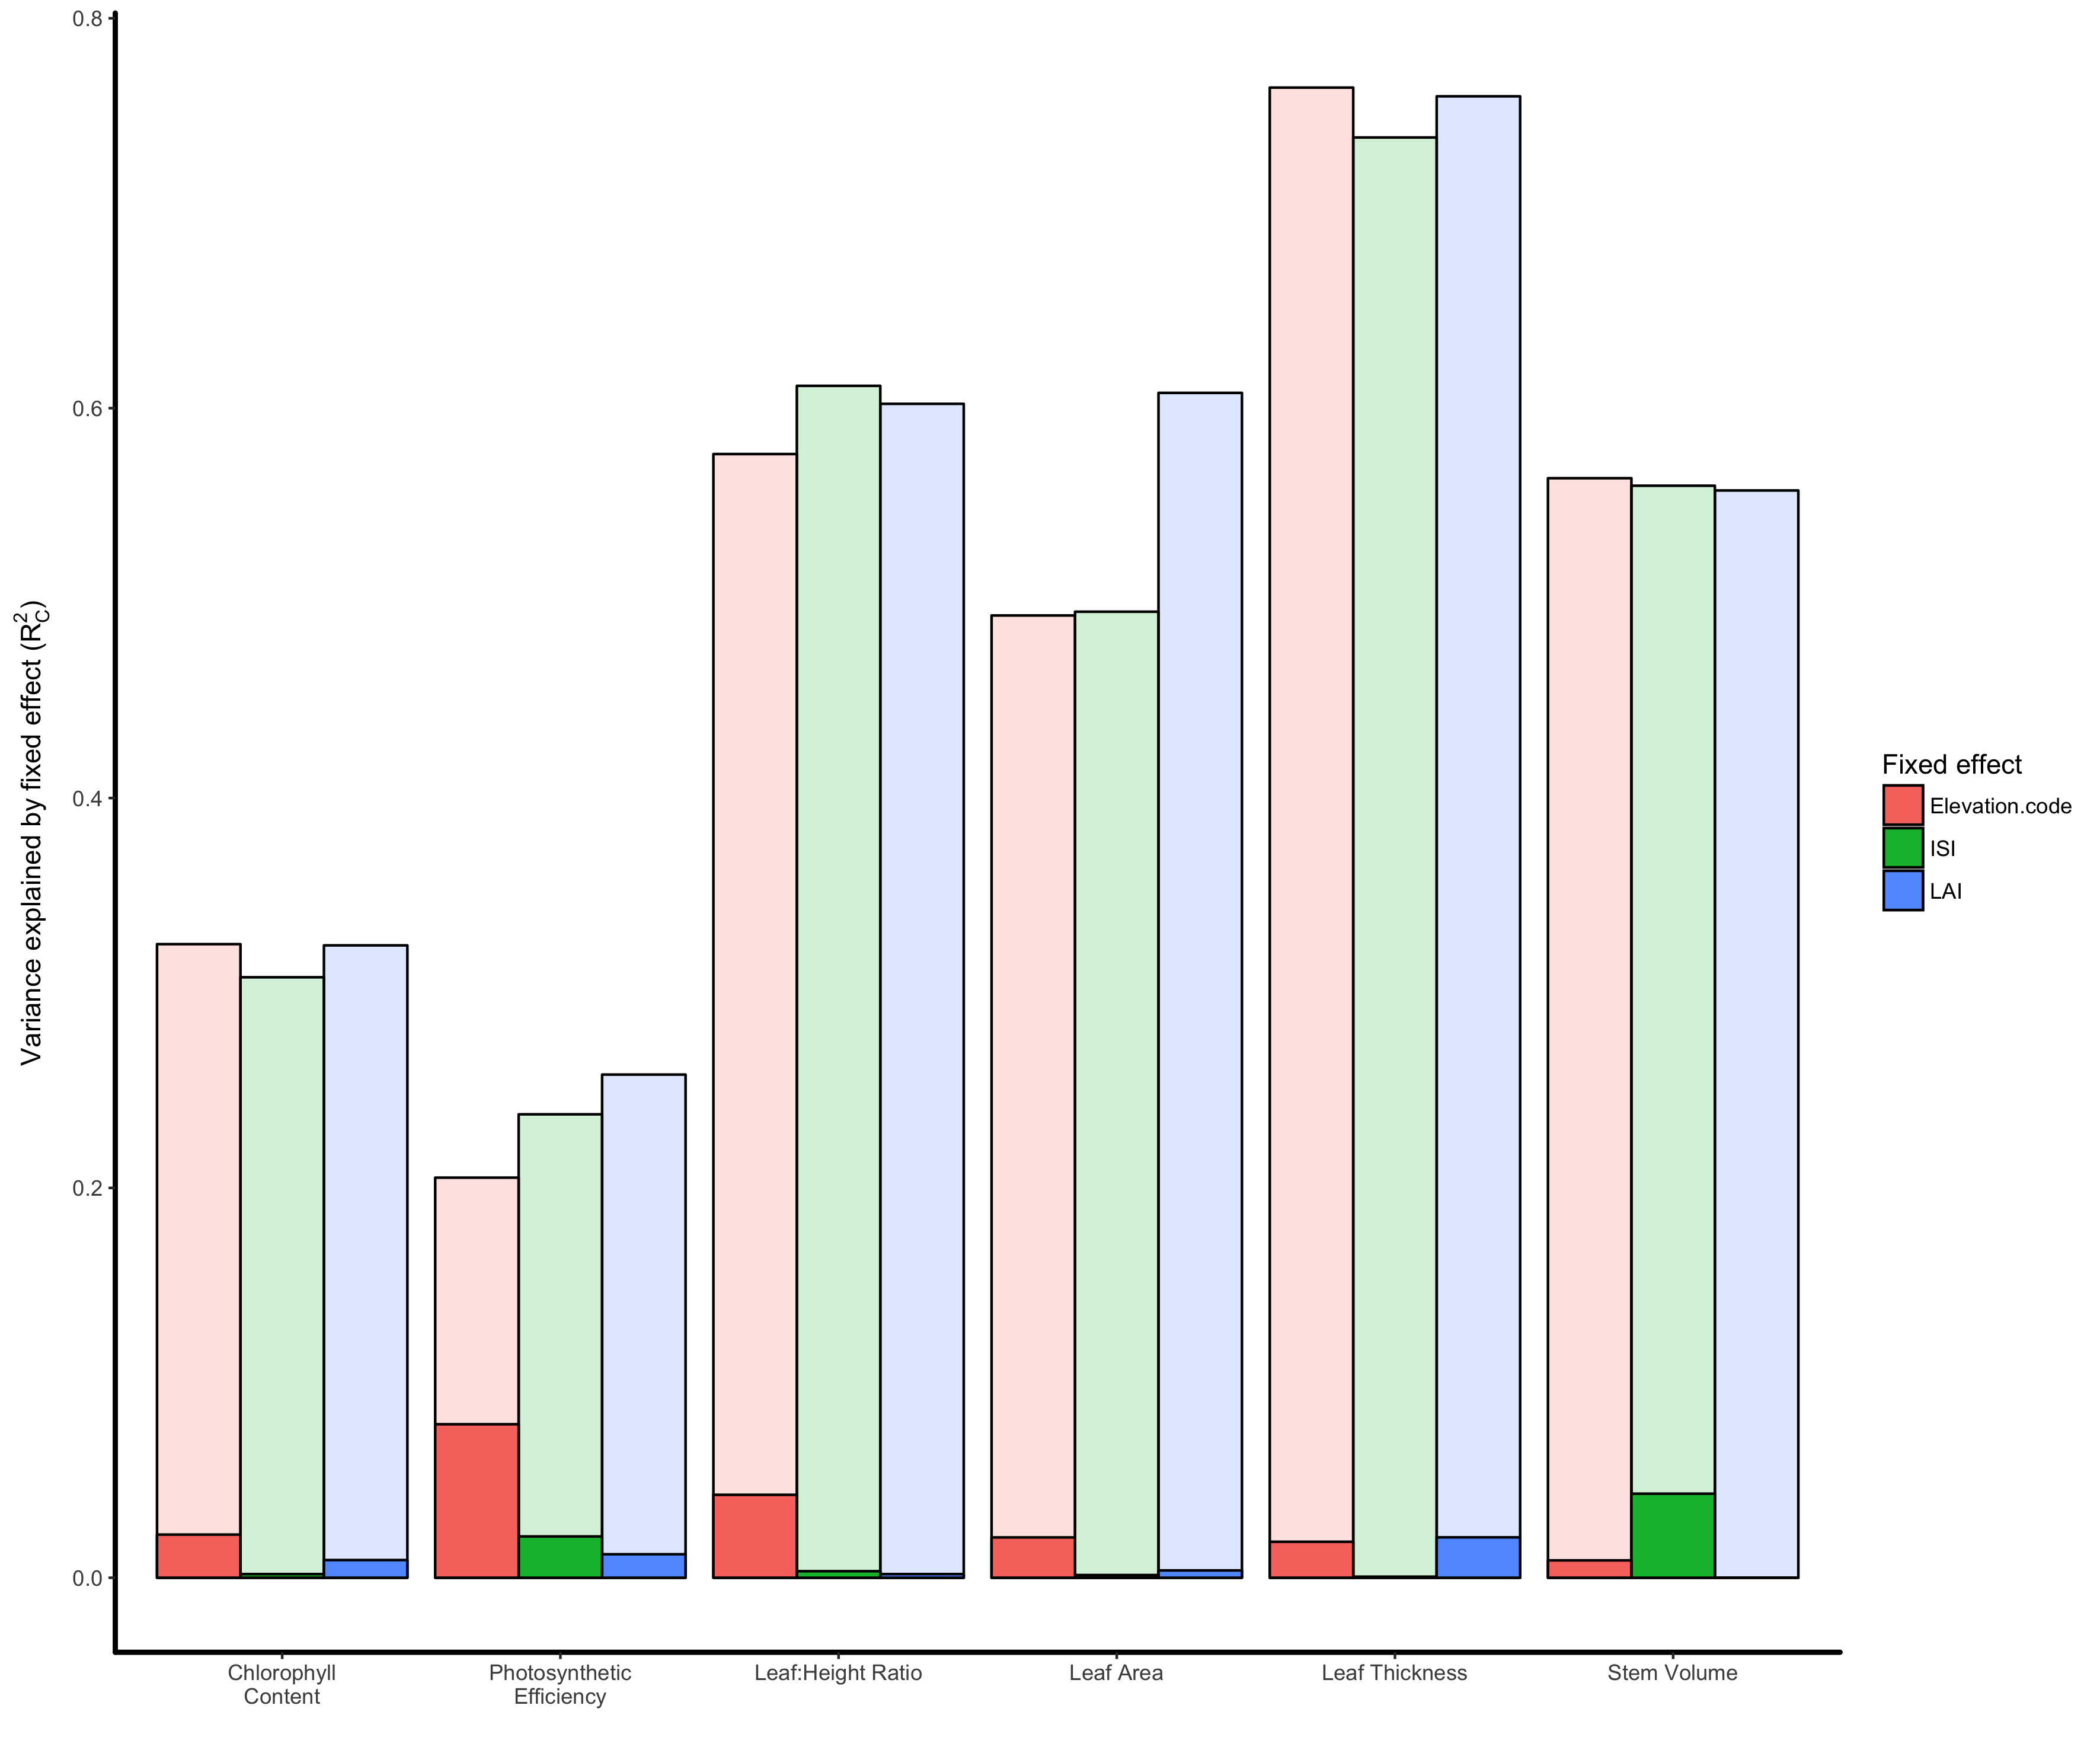
\includegraphics[width=\textwidth]{r2plot_ggplot}
\centering
\caption{The variance explained by each single fixed effect model. The pale bars indicate the variance explained by the whole model while the bold bars indicate the variance explained just by the fixed effect in the model.}
\label{fig:r2plot_ggplot}
\end{figure}

Table \ref{tab:best_fit_multi} shows the fixed effects and model fit measures from the best fitting multiple fixed effect models used to predict plant traits. For plant traits where one or more of the single fixed effect models was better when using a random slope (Figure \ref{fig:traits_dAIC}), the species slopes were allowed to vary for those fixed effects (Table \ref{tab:best_fit_multi}) in some model iterations. 

All of the best models except the one predicting SPAD included elevation as a fixed effect alongside competition variables. All of the best models were better than a model using only elevation (Appendix IV). The best models for leaf:height ratio, leaf area and stem volume used random slopes for all the fixed effects identified as varying among species in the single predictor models. The fixed effects in the multiple fixed effect models still accounted for a small percentage of the variation in plant traits, ranging from 0.4\% (SPAD), to 17.3\% (stem volume).

When multiple fixed effects were used in a model, the standard errors surrounding the slopes of those fixed effects were reduced (Figure \ref{fig:fix_eff}, Appendix II). The effect of herbaceous plant abundance became larger in the multiple fixed effects model compared to the single fixed effect model. The best LMM for SPAD was no better than a random effects model ($\Delta$AIC\textsubscript{r} = -1.0) and was 14.2\% likely to be better than the next best model, which included only elevation ($W_i$ = 0.142).

\subsection{Effects of competition on plant traits}

Linear mixed effect models of the relationship between adult tree competition variables and plant traits outperformed equivalent random effect models in \todo{15/24 cases}, \textit{i.e.} those with a $\Delta$AIC\textsubscript{r}>2. However, the competition variables only accounted for a small percentage of the variance in each plant trait. The the highest $R_M^2$ in these single fixed effects models was the effect of Iterative Seedling Index on stem volume ($R_M^2$ = 4.3\%), despite the model as a whole explaining 56\% of the variation in stem volume. A similar effect is seen in all the other single fixed effect models, suggesting that unmeasured site specific effects are responsible for a large portion of the variation in plant traits.

The best fitting multiple fixed effect models all included the effects of elevation, Iterative Seedling Index and Leaf Area Index to explain variation in plant traits, except leaf chlorophyll content, which only included Leaf Area Index. 


\section*{Discussion}

\section*{Conclusion}


Forest structure based competition affects physiological stress independently of elevation

%--------------------------------------------------------------
\end{document}
%--------------------------------------------------------------
